Vibrational spectroscopy links molecular structure to experimentally observable signals. Infrared (IR) absorption and Raman scattering probe the same molecular normal modes through different responses: changes in dipole moment and polarizability, respectively~\cite{Hashimoto_2019,Chang_2022,Meng_2025}. Their selection rules make the two modalities complementary. A vibration that is weak or inactive in one spectrum may be prominent in the other; in centrosymmetric molecules, IR and Raman activity are mutually exclusive. Access to both modalities can therefore aid band assignment and the characterization of molecular bonding and symmetry~\cite{yuan2025qme14s,wang2025diffspectra,wang2025molspectra}.

Paired measurements are nevertheless difficult to obtain at scale. Public IR and Raman libraries have developed largely independently, and Raman acquisition can be limited by weak scattering, fluorescence and sample damage~\cite{Chan_2005,Sasmaz_2015,Wei_2015,Shipp_2017}. Quantum-chemical calculations provide paired spectra, but their cost and sensitivity to computational approximations, molecular conformation and environment limit direct correspondence with measurements~\cite{zou2023deep,liang2025dataset,Laury_2012,Barone_2014,Bloino_2015}. Predicting one modality from the other could help complete spectral records when paired data are unavailable. Such predictions must be interpreted as learned estimates: selection rules can hide information in the source, so the target spectrum is not generally determined by a simple rescaling of source intensities.

Cross-modal learning must resolve narrow peaks while using relationships across the wavenumber axis. Existing work has explored learned IR--Raman correspondence~\cite{yang2024cross}, alongside broader approaches to learning from molecular spectra~\cite{lu2025vib2mol,cai2025deep,kanakala2024spectra,alberts2025setting,su2025language}. Two questions remain central to this task: how well a learned mapping transfers across chemical and measurement domains, and whether translation produces representations useful beyond spectral reconstruction. The shared molecular origin of the two modalities motivates testing cross-modal prediction as an objective for molecular representation learning~\cite{zhu2026spectrogen}.

Here we introduce \mname, a conditional flow-matching framework for bidirectional IR--Raman translation (Fig.~\ref{fig:pipeline}). A one-dimensional Transformer learns a source-conditioned velocity field over ordered wavenumber sequences. Peak weighting, derivative matching and local optimal transport emphasize spectral morphology, while deterministic integration produces a target prediction and intermediate model states. We evaluate translation on three computed-spectrum benchmarks, transfer from the ViBench-QM9 source domain to seven held-out domains, and performance under experimental-input and cross-library shifts. We also test whether frozen translation-trained features support molecular-descriptor prediction. These evaluations distinguish reconstruction accuracy, domain transfer and representation utility, while treating the learned trajectory as a computational path rather than physical molecular dynamics.

\begin{figure}[htbp]
    \centering
    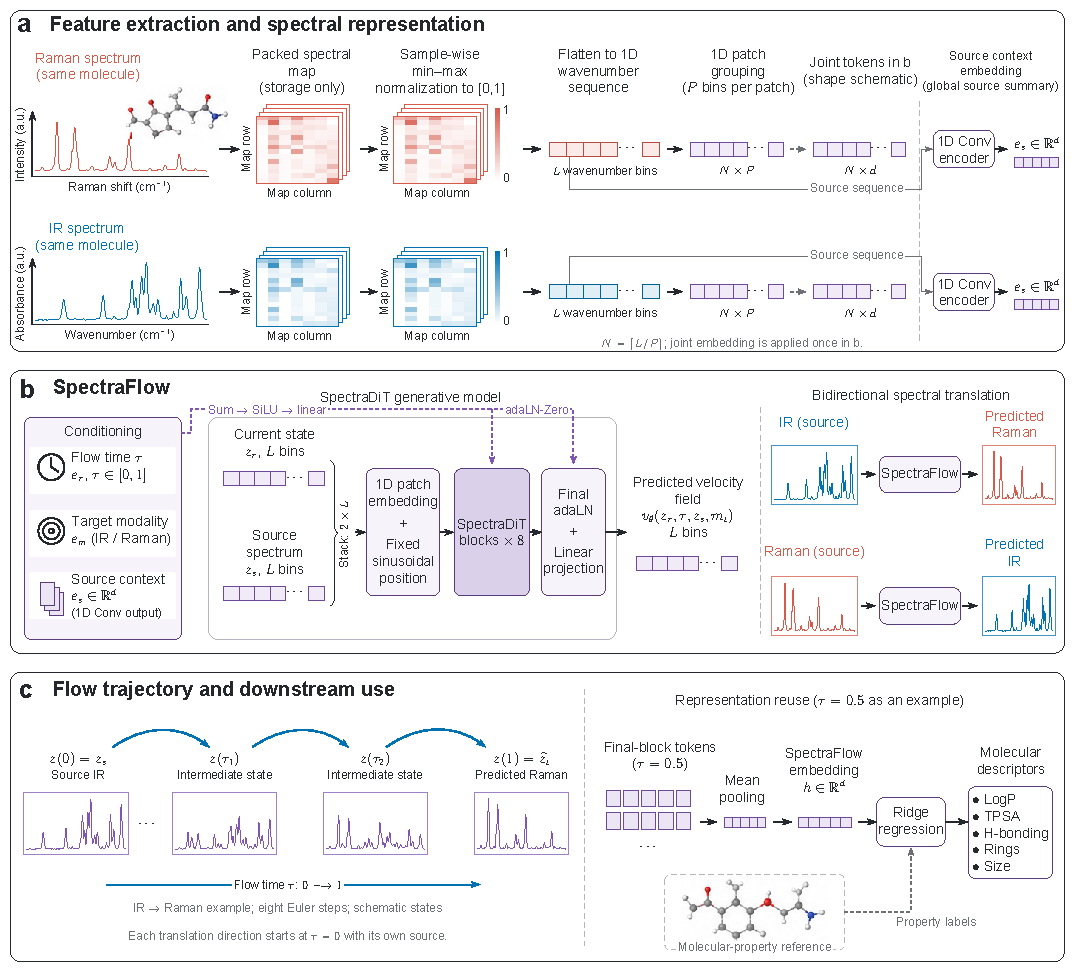
\includegraphics[width=\linewidth]{figs/Figure_1_reference_tikz.pdf}
    \caption{\textbf{Overview of \mname\ for bidirectional IR--Raman translation.}
    \textbf{a,} Paired spectra are normalized sample-wise and flattened into ordered wavenumber sequences; heatmaps depict per-spectrum storage grids. Patch grouping and token dimensions are schematic. The learned joint embedding is applied once to the stacked channels in b. A separate one-dimensional convolutional encoder summarizes the source sequence.
    \textbf{b,} The current state and source spectrum, $[z_\tau,z_s]$, pass through a joint one-dimensional patch embedding, fixed sinusoidal positions, eight SpectraDiT blocks and an output head. Summed time, modality and source-context embeddings undergo SiLU activation and an affine projection before conditioning adaptive layer normalization. Separate checkpoints implement the two translation directions.
    \textbf{c,} Four schematic states illustrate IR$\rightarrow$Raman translation with eight Euler steps. Integration starts from the source at $\tau=0$ and ends at the predicted target at $\tau=1$. Final-block tokens at the source-generated midpoint $\tau=0.5$ are mean-pooled for ridge-regression probes. Molecular structures supply property labels, not translator inputs. Spectra, heatmaps and intermediate states are schematic.}
    \label{fig:pipeline}
\end{figure}
